\documentclass{article}
\usepackage[paperwidth=594mm,paperheight=841mm,top=16mm,bottom=16mm,left=19mm,right=19mm]{geometry}
\usepackage[T1]{fontenc}
\usepackage{helvet}
\usepackage{xcolor}
\usepackage{graphicx}
\usepackage{ragged2e}
\usepackage{microtype}
\usepackage{tabularx}
\usepackage{array}
\usepackage{enumitem}

\renewcommand{\familydefault}{\sfdefault}
\definecolor{ink}{HTML}{182E42}
\definecolor{blue}{HTML}{007AC3}
\definecolor{accent}{HTML}{C55A11}
\definecolor{softblue}{HTML}{EAF5FA}
\definecolor{softorange}{HTML}{FBEFE7}
\definecolor{rulegray}{HTML}{CBD5DC}
\color{ink}
\pagestyle{empty}
\setlength{\parindent}{0pt}
\setlength{\parskip}{2.5mm}
\setlength{\tabcolsep}{3mm}
\renewcommand{\arraystretch}{1.22}
\hyphenpenalty=10000
\exhyphenpenalty=10000
\setlist[itemize]{leftmargin=8mm,itemsep=1.6mm,topsep=1mm,parsep=0mm}

\newcommand{\TargetAccuracy}{50.0\%}
\newcommand{\ContextAccuracy}{55.5\%}
\newcommand{\BertAccuracy}{67.1\%}
\newcommand{\AccuracyGain}{11.6}
\newcommand{\BertMacroF}{66.7\%}
\newcommand{\ContextMacroF}{55.1\%}
\newcommand{\DifferenceLower}{-16.9}
\newcommand{\DifferenceUpper}{-6.6}
\newcommand{\ValidationCount}{638}
\newcommand{\SelectionHash}{debfd61b068f22ea1a737f238bd90ea4fb8bf44f675907e428949b559a0bb309}
\newcommand{\BertOnlyCount}{178}
\newcommand{\StaticOnlyCount}{104}
\newcommand{\BertErrorCount}{210}

% Author details supplied by the user on 2026-09-13.
\newcommand{\FirstAuthor}{Choudhary Prashant Santosh}
\newcommand{\FirstEnrollment}{1910474}
\newcommand{\SecondAuthor}{Rahul Khunt}
\newcommand{\SecondEnrollment}{1911272}


\newcommand{\bodyfont}{\fontsize{25}{31}\selectfont}
\newcommand{\smallfont}{\fontsize{22}{27}\selectfont}
\newcommand{\reffont}{\fontsize{17}{21}\selectfont}
\newcommand{\sectiontitle}[1]{%
  {\fontsize{31}{37}\selectfont\bfseries\textcolor{blue}{#1}\par}\vspace{1mm}}
\newcommand{\numbertitle}[2]{%
  {\fontsize{31}{37}\selectfont\bfseries\textcolor{accent}{#1}\hspace{2.5mm}\textcolor{blue}{#2}\par}\vspace{1mm}}
\newcommand{\questiontitle}[2]{%
  {\fontsize{18}{22}\selectfont\bfseries\textcolor{accent}{#1}\par}\vspace{-0.5mm}%
  {\fontsize{31}{37}\selectfont\bfseries\textcolor{blue}{#2}\par}\vspace{1mm}}
\newcommand{\divider}{\par\vspace{1mm}{\color{rulegray}\rule{\linewidth}{0.6pt}}\par\vspace{2mm}}
\newcommand{\ResultCallout}[2]{%
  \begin{minipage}[t]{0.31\linewidth}\centering
  {\fontsize{42}{48}\selectfont\bfseries\textcolor{blue}{#1}\par}
  {\fontsize{21}{26}\selectfont #2}
  \end{minipage}}
\newcommand{\PosterHeader}[2]{%
  \begin{center}
  \setlength{\parskip}{0.7mm}
  
\includegraphics[width=65mm]{../assets/university-trier.pdf}\par
  \vspace{2mm}
  {\fontsize{45}{51}\selectfont\bfseries #1\par}
  {\fontsize{27}{33}\selectfont\textcolor{blue}{#2}\par}
  \vspace{2mm}
  \begin{minipage}[t]{0.40\textwidth}\centering
  {\fontsize{26}{31}\selectfont\bfseries\FirstAuthor{}}\par
  {\fontsize{22}{27}\selectfont Enrollment no.\ \FirstEnrollment{}}
  \end{minipage}\hspace{5mm}%
  \begin{minipage}[t]{0.40\textwidth}\centering
  {\fontsize{26}{31}\selectfont\bfseries\SecondAuthor{}}\par
  {\fontsize{22}{27}\selectfont Enrollment no.\ \SecondEnrollment{}}
  \end{minipage}\par
  \vspace{1mm}
  {\fontsize{22}{27}\selectfont University of Trier\quad MSc Natural Language Processing\quad Trends in Natural Language Processing}
  \end{center}
  \vspace{-4mm}\divider}
\newcommand{\ReferencesBlock}{%
  {\color{rulegray}\rule{\textwidth}{0.6pt}}\par\vspace{1mm}
  {\reffont\textbf{References}\par\vspace{0.5mm}
  \begin{minipage}[t]{0.32\textwidth}\RaggedRight
  [1] Pilehvar \& Camacho-Collados (2019). \textit{WiC}. NAACL.\par
  [2] Pennington, Socher \& Manning (2014). \textit{GloVe}. EMNLP.
  \end{minipage}\hfill
  \begin{minipage}[t]{0.32\textwidth}\RaggedRight
  [3] Devlin et al. (2019). \textit{BERT}. NAACL.\par
  [4] Camacho-Collados \& Pilehvar (2018). \textit{From Word to Sense Embeddings}. JAIR.
  \end{minipage}\hfill
  \begin{minipage}[t]{0.32\textwidth}\RaggedRight
  [5] Loureiro et al. (2021). \textit{Language Models for Word Sense Disambiguation}. Computational Linguistics.\par
  [6] Haber \& Poesio (2021). \textit{Polysemy and Homonymy in Contextualised Language Models}. Findings of EMNLP.
  \end{minipage}}}


\begin{document}
\bodyfont
\PosterHeader{Static vs Contextual Embeddings for Lexical Ambiguity}{WiC evaluation in eight steps}

\noindent
\begin{minipage}[t][530mm][s]{0.485\textwidth}\vspace{0pt}\RaggedRight
\numbertitle{1}{Introduction}
\begin{itemize}
\item \textbf{Lexical ambiguity} means that words such as \textbf{bank} have more than one meaning.
\item Static GloVe uses one vector for every occurrence [2].
\item Contextual BERT changes the vector with the sentence [3].
\item \textbf{Aim:} test which representation captures sense differences better.
\end{itemize}

\vfill
\numbertitle{2}{Definitions}
\begin{itemize}
\item \textbf{Homonymy:} unrelated meanings. \textbf{Polysemy:} related meanings [6].
\item \textbf{Embedding:} a word represented as a numerical vector.
\item \textbf{Cosine similarity:} how closely two vector directions align.
\item \textbf{WiC task:} does the same word have the same meaning in two sentences? [1]
\end{itemize}

\vfill
\numbertitle{3}{Related work}
\begin{itemize}
\item WordNet and dictionary-based word sense disambiguation.
\item Multi-sense embeddings with several vectors per word [4].
\item Contextual models such as ELMo and BERT.
\item WiC as a context-sensitive benchmark, introduced in 2019 [1].
\end{itemize}

\vfill
\numbertitle{4}{Hypotheses}
\begin{itemize}
\item H1: the static target diagnostic remains at chance.
\item H2: nearby GloVe context gives a small improvement.
\item H3: frozen BERT beats GloVe context without fine-tuning.
\end{itemize}
\end{minipage}\hfill
\begin{minipage}[t][530mm][s]{0.485\textwidth}\vspace{0pt}\RaggedRight
\numbertitle{5}{Methodology}
\begin{itemize}
\item WiC: \TrainCount{} train, \ValidationCount{} validation and \TestCount{} public test pairs without public labels.
\item Systems: GloVe target, GloVe context \SelectedContextWindow{}, BERT last-four-layer mean.
\item Cosine threshold and settings selected on training data only.
\item Validation used once. \BootstrapResamples{} paired bootstrap resamples.
\end{itemize}

\vfill
\numbertitle{6}{Results}
\noindent
\ResultCallout{\TargetAccuracy}{GloVe target}\hfill
\ResultCallout{\ContextAccuracy}{GloVe context}\hfill
\ResultCallout{\BertAccuracy}{BERT}

\vspace{2mm}
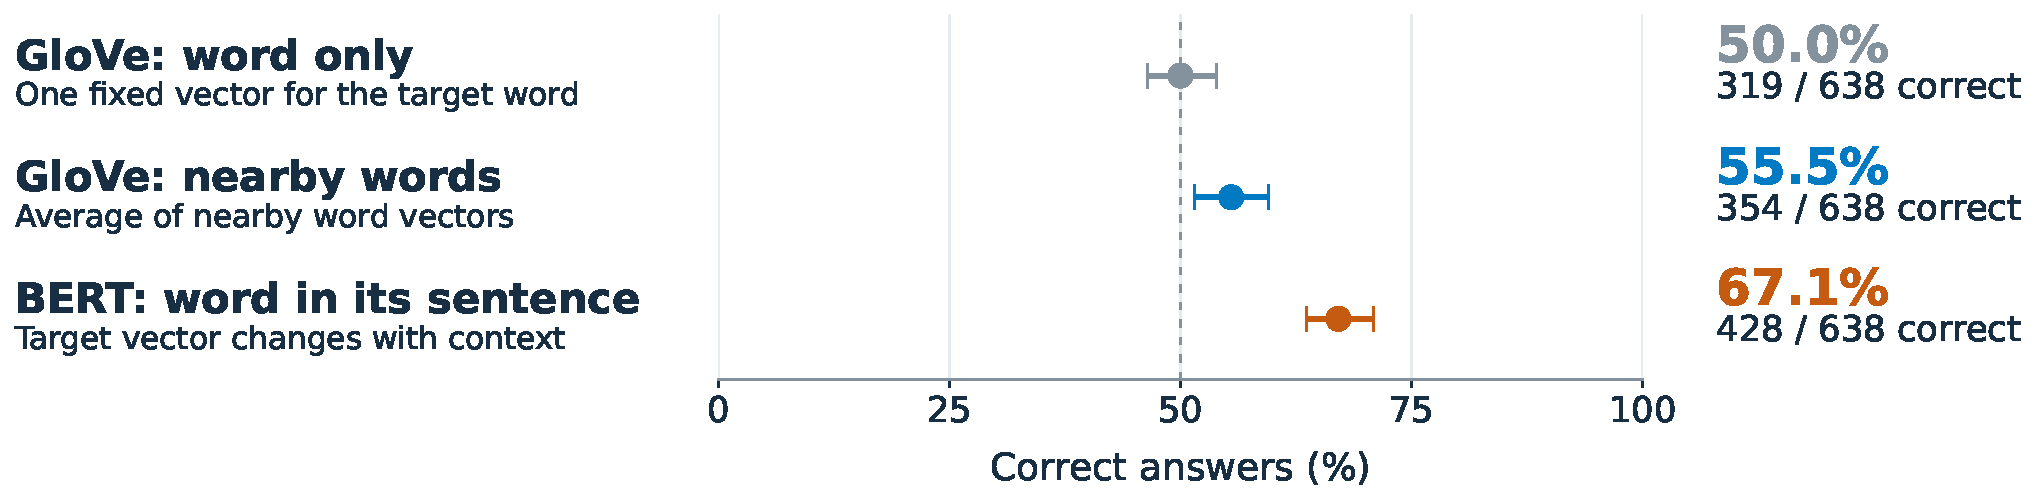
\includegraphics[width=\linewidth]{../../figures/poster_accuracy.pdf}

{\smallfont BERT gains \AccuracyGain{} points over GloVe context. Paired 95\% interval: \GainLower{} to \GainUpper{}. BERT macro F1 is \BertMacroF{} and ROC-AUC is \BertAuc{}. Layer \BestAccuracyLayer{} reaches 66.6\%, while layer \FinalLayerNumber{} reaches 63.6\%.}

\vfill
\numbertitle{7}{Error analysis}
\begin{itemize}
\item BERT right and GloVe wrong: \BertOnlyCount{}. GloVe right and BERT wrong: \StaticOnlyCount{}.
\item BERT same-sense recall: \BertSameRecall{}. Different-sense recall: \BertDifferentRecall{}.
\item GloVe context same-sense recall: \ContextSameRecall{}. Different-sense recall: \ContextDifferentRecall{}.
\item BERT errors: \BertErrorCount{} of \ValidationCount{}.
\end{itemize}

\vfill
\numbertitle{8}{Conclusion}
BERT captures sense differences better than GloVe on this frozen WiC protocol. It still reaches only \BertAccuracy{}. The evidence comes from one small English validation set, one frozen BERT model and a simple GloVe baseline.
\end{minipage}

\vfill
\ReferencesBlock
\end{document}
